\documentclass[11pt,letterpaper]{article}

\usepackage[letterpaper,margin=0.8in,nohead]{geometry}

\usepackage[colorlinks]{hyperref}
\usepackage{url}
\usepackage{breakurl}

\hypersetup{
	colorlinks,
	linkcolor={red},
	citecolor={red},
	urlcolor={blue}
}

\usepackage{verbatim}
\usepackage{fancyvrb}
\usepackage{scrextend}
\usepackage{enumitem}
\usepackage{url}
\usepackage{tabularx}
\usepackage[dvipsnames]{xcolor}

\usepackage{caption}
\usepackage{graphicx}
\usepackage{subcaption}

\usepackage{changepage}   % for the adjustwidth environment

\newenvironment{answer}{\em \color{blue} \begin{adjustwidth}{1cm}{1cm}}{\end{adjustwidth}}

% math
\usepackage{amsthm,amsmath}
\usepackage{amsfonts}

\newcommand{\mc}[1]{\mathcal{#1}}	% Mechanisms / Algorithms
\newcommand{\rv}[1]{\mathbf{#1}}    % Random variable

\newcommand{\pr}[1]{\mathrm{Pr}\{#1\}} % Probability

\newtheorem{corollary}{\bf Corollary}%[theorem]
\newtheorem{lemma}{\bf Lemma}%[theorem]
\newtheorem{definition}{\bf Definition}%[section]

\newtheorem{observation}{\bf Observation}%[theorem]

% load cleveref last!
\usepackage[capitalise]{cleveref}


\begin{document}
	
	\title{EN4720: Security in Cyber-Physical Systems \\ Exercise --- Authorization}
	
	%% This is an individual assignment!!
	%% TODO: put your name and index number here here!
	\author{ \textcolor{blue}{Name: John Doe} \\ \textcolor{blue}{Index No: XXXXX}}
	
	\maketitle
	
	\begin{center}
		\color{red}\bf This is an individual exercise! \\ Due Date: 19 May 2023 by 11.59 PM
	\end{center}
	
	\vspace{1in}
	
	This exercise has to be carried out using a Linux-based PC/virtual machine. Read all the instructions and questions before attempting the exercise. Add answers under each question in the Questions section and submit the resulting PDF.
	
	\subsection*{Instructions}
	
	\begin{enumerate}
		\item Understand how linux users and groups work.
		
		\item Understand how linux file ownership and permissions work.
		
		\item Answer the questions given below.
		
	\end{enumerate}
	
	\newpage
	
	\section*{Questions}
	
	For all the questions in this section, add a screenshot of the terminal (including all the commands you ran to perform the task) unless specified otherwise. The evaluator should be able to see each step that you followed to perform each task. In all screenshots, the areas marked (which are unique to your terminal display) in Figure 1 (the sample answer to Question 1) must be visible.
	
	\begin{enumerate}
		
		\item View the currently logged in user.
		
		\begin{figure}[h]
			\centering
			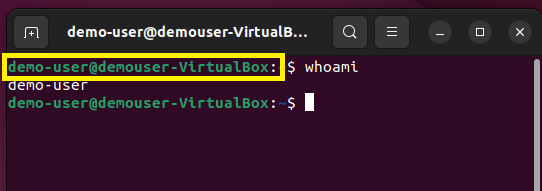
\includegraphics[width=0.65\columnwidth]{images/ex4-sample-terminal-output.png}
			\caption{Sample Terminal Output} \label{fig:sample-terminal-output}
		\end{figure}
		
		\item Create a sub directory as excercise4. Create a text file resolutions.txt with “Hello World” text in the file and store the file in the newly created directory as exercise4/resolutions.txt. Dump the file to the terminal using the \texttt{cat} command.
		
		\begin{answer}
			%% TODO: Add answer here
			Your answer here
		\end{answer}
		
		\item Create two new user accounts as \textcolor{magenta}{alice} and \textcolor{magenta}{\textcolor{magenta}{bob}}.
		
		\begin{answer}
			%% TODO: Add answer here
			Your answer here
		\end{answer}
		
		\item Create a group as \textcolor{ForestGreen}{friends} and add \textcolor{magenta}{alice} and yourself (currently logged in user) to the group \textcolor{ForestGreen}{friends}
		
		\begin{answer}
			%% TODO: Add answer here
			Your answer here
		\end{answer}
		
		\item Make sure your (currently logged in user's) home directory has execute permissions for all the users.
		
		\begin{answer}
			%% TODO: Add answer here
			Your answer here
		\end{answer}
		
		\item Become (log in as) one of your new user accounts (\textcolor{magenta}{alice} or \textcolor{magenta}{bob}). You can simply \texttt{su -} to the alternate user.
		
		\begin{answer}
			%% TODO: Add answer here
			Your answer here
		\end{answer}
		
		
		\item As the new user, confirm that you can view the file by dumping the content to the terminal. Try adding a new item to the resolutions.txt file. Why can’t you modify the file as the new user?
		
		\begin{answer}
			%% TODO: Add answer here
			Your answer here
		\end{answer}
		
		\item Note that the permissions on a newly created file allow all users on the system to read the file. Assume that you want to keep resolutions.txt file private. Modify the file's permissions, such that read access for others is removed. 
		
		\begin{answer}
			%% TODO: Add answer here
			Your answer here
		\end{answer}
		
		
		\item Using the other new account (if you used \textcolor{magenta}{alice} before, now use \textcolor{magenta}{bob}), confirm that other users on the system are not able to read your resolutions.txt file by trying to dump the file to the terminal.
		
		\begin{answer}
			%% TODO: Add answer here
			Your answer here
		\end{answer}
		
		\item Compose a short shopping list in your preferred text editor, or using the command line. Store the file as exercise4/shopping.txt. Change the group owner of the file to \textcolor{ForestGreen}{friends}.
		
		\begin{answer}
			%% TODO: Add answer here
			Your answer here
		\end{answer}
		
		\item As the alternate user \textcolor{magenta}{alice}, confirm that you can view the file. Also, note that you can modify the file, by adding an additional item to the shopping list. Dump the file content to the terminal to show that the new item is added.
		
		\begin{answer}
			%% TODO: Add answer here
			Your answer here
		\end{answer}
		
		\item Recall that your other new account (\textcolor{magenta}{bob}) is not a member of the group \textcolor{ForestGreen}{friends}. Try becoming \textcolor{magenta}{bob} and repeat the previous steps. You should be able to view, but not modify, the file.
		
		\begin{answer}
			%% TODO: Add answer here
			Your answer here
		\end{answer}
		
		\vspace{5mm}
		
		Provide analytical answers to the questions below. Screenshots are not required.
		
		\item What are the challenges that organizations face during the cyber security authorization process, and how can they be overcome?
		
		\begin{answer}
			%% TODO: Add answer here
			Your answer here
		\end{answer}
		
		\item How do different cyber security authorization frameworks differ from one another, and what are the key considerations that organizations should take into account when choosing a framework to follow?
		
		\begin{answer}
			%% TODO: Add answer here
			Your answer here
		\end{answer}
		
		\item What are the most common vulnerabilities that may be identified during the cyber security authorization process, and how can organizations address them?
		
		\begin{answer}
			%% TODO: Add answer here
			Your answer here
		\end{answer}
		
	\end{enumerate}
	
\end{document}